\specsection{2.6 Сформулировать определение случайного вектора и функции распределения вероятностей случайного вектора. Сформулировать определение непрерывного случайного вектора и доказать свойства плотности распределения вероятностей для двумерного случайного вектора.}

Пусть $(\Omega, \beta, P)$ -- вероятностное пространство

$x_1(\omega),...,x_n(\omega)$ - сл. вел. заданные на этом пространстве

\OPR $n$-мерным случ. вектором наз. кортеж $\overrightarrow{x}=(x_1(\omega),...,x_n(\omega))$

\OPR Ф-ей распределения $n$-мерного случ. вектора $(x_1,...,x_n)$ наз. отображение 

$F:\R^n\rightarrow\R$, которое определено усл-м $F(x_1,...,x_n)=P\{X_1<x_1,...,X_n<x_n\}$

\OPR Сл. вектор $(x_1,...,x_n)$ наз. непрерывным, если существует ф-ия $f(x_1,...,x_n)$ такая что $F(x_1,...,x_n)=\intl_{-\infty}^{x_1}dt_1\intl_{-\infty}^{x_2}dt_2...\intl_{-\infty}^{x_n}f(t_1,...,t_n)dt_n$

\OPR 1) $f(x_1,...,x_n)$ наз. (совместной) плотностью распред. вер-ей сл. в-ра $(x_1,...,x_n)$

2) предполагается, что указанный несобств. интеграл сходится для всех $(x_1,...,x_n)\in\R^n$

Свойства двумерных непрерывных случайных векторов
\begin{enumerate}[topsep=0pt, leftmargin=20pt, noitemsep, label=\arabic*\degree]
	\item $f(x, y) \geq 0$
	
	\item $P\{a_1\leq x < b_1, a_2\leq y < b_2\}=\intl_{a_1}^{b_1}dx\intl_{a_2}^{b_2}f(x,y)dy$
	
	\item $\iintl_{R^2}f(x,y)dxdy=1$
		
	\item $P\{a_1\leq x<a_1+\varDelta x, a_2\leq y<a_2+\varDelta y\}\approx f(a_1, a_2)\varDelta x\varDelta y$, где $(a_1,a_2)$ - т. непр. ф-ии $f(x,y)$
	
	\item Для любого наперёд заданного значения $(x\degree, y\degree)~P\{(x,y)=(x\degree, y\degree)\}=0$
	
	\item $P\{(x,y)\in D\}=\iintl_{D}f(x,y)dxdy$
	
	\item $\intl_{-\infty}^{+\infty}f(x,y)dy = f_X(x)~~~\intl_{-\infty}^{+\infty}f(x,y)dx = f_Y(y)$
	
	\item [] Доказательства
	\setcounter{enumi}{0}
	
	\item $f(x,y)=F'(x,y)$, т.к. $F(x,y)$ -- неуб. ф-ия, то $F'(x,y)\geq 0\Rightarrow f(x,y)\geq 0$

	\item [-..-] \textcolor{red}{ниже представлено (2-5) для одномерной, надо переделать по наналогии}
	
	\item По свойству функции распределения $P\{x_1\leq X \leq x_2\}=F(x_2)-F(x_1)=|$ т.к. $F(x)$ -- первообразная для $f(x)|\stackrel{\text{ф-ла Ньютона-Лейбница}}{=}\intl_{x_1}^{x_2}f(x)dx$
	
	\item $\intl_{-\infty}^{+\infty}f(x)dx\stackrel{\text{св-во 2\degree}}{=}F(+\infty)-F(-\infty)=1-0=1$
	
	\item $P\{x_0\leq X \leq x_0+\varDelta x\}=F(x_2)=F(x_1)\stackrel{\text{th Лагранжа (f непрер.)}}{=}f(\xi)\varDelta x$, где $\xi\in(x_0, x+\varDelta x)$
	\item [] ~
	\item []
	\begin{minipage}{\linewidth}
		\centering
		\begin{minipage}{0.25\linewidth}
			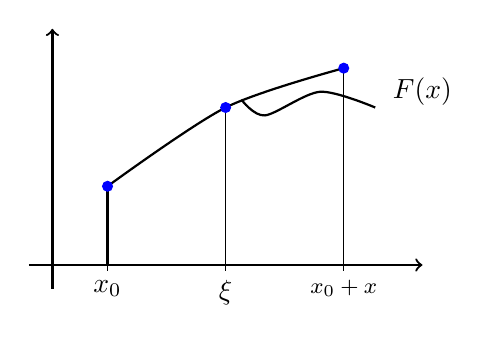
\begin{tikzpicture}
				\draw[thick,->] (0,0) -- (5,0);
				\draw[thick,->] (0.3,-0.3) -- (0.3,3);
				\draw[thick] plot [smooth] coordinates {(1,1) (2.5,2) (4, 2.5)};
				
				\draw (1,2pt) -- (1,-2pt) node[anchor=north] {$x_0$};
				\draw[thick,-] (1,0) -- (1,1);
				\fill[blue,thick] (1,1) circle (2pt);
				
				\draw (2.5,2pt) -- (2.5,-2pt) node[anchor=north] {$\xi$};
				\draw[thin,-] (2.5,0) -- (2.5,2);
				\fill[blue,thick] (2.5,2) circle (2pt);
				
				\draw (4,2pt) -- (4,-2pt) node[anchor=north] {\footnotesize{$x_0+\varDelta x$}};
				\draw[thin,-] (4,0) -- (4,2.5);
				\fill[blue,thick] (4,2.5) circle (2pt);
				
				\draw (5,2.5) node[anchor=north] {$F(x)$};
				
				\draw[thick] plot [smooth] coordinates {(2.7,2.1) (3,1.9) (3.7, 2.2) (4.4,2)};
	\end{tikzpicture}
		\end{minipage}
		\hspace{0.05\linewidth}
		\begin{minipage}{0.65\linewidth}
			Т.к. $\varDelta x$ <<мала>>, а $f$ непрерывна, то $f(\xi)\approx f(x_0)$
			
			~
			
			$P\{x_0\leq X\leq x_0+\varDelta x\}\approx f(x_0)\varDelta x$
		\end{minipage}
	\end{minipage}
	
	\item $P\{X=x_0\}=\liml_{\varDelta x \rightarrow 0}P\{x_0\leq X\leq x_0+\varDelta x\}=\liml_{\varDelta x \rightarrow 0}f(\xi)\varDelta x\stackrel{\text{f непр. }\Rightarrow \text{ огр.}}{=}0$
	
	\item Является обобщением $2\degree$ (без док-ва)
	
	\item $F_X(x)=F(x,+\infty)\stackrel{\text{непр. сл. в-ра.}}{=}\intl_{-\infty}^{+\infty}dt_1\intl_{-\infty}^{+\infty}f(t_1,t_2)dt_2$
	\item [] продиф. обе части по $x:~F'_X(x)=\tfrac{dF_X(x)}{dx}=f_X(x)=$
	\item [] $=|\text{x - точка непр.}~f_X \Rightarrow \text{по th о произвольной интеграла с верхним пределом}|=$
	\item [] $=\intl_{-\infty}^{+\infty}f(x,t_2)dt_2$ ~для $f_Y$ аналогично
	
\end{enumerate}

\clearpage
